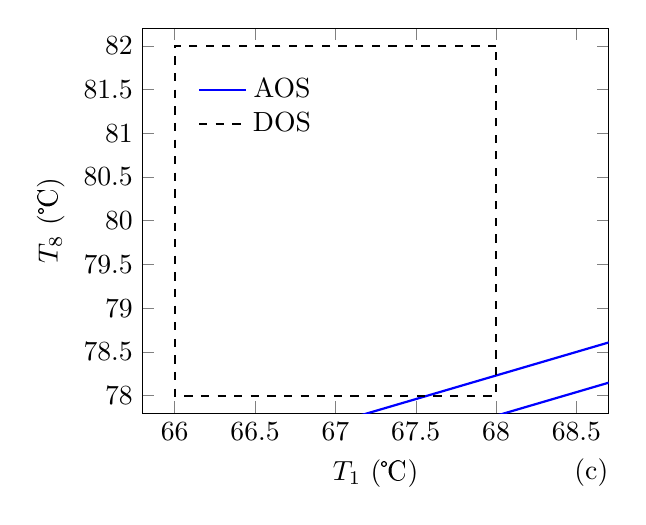
\begin{tikzpicture}
  \begin{axis}[
    width=7.5cm,
    xlabel=$T_1$~(\textcelsius),
    ylabel=$T_8$~(\textcelsius),
    xmin=65.8,xmax=68.7,ymin=77.8,ymax=82.2,
    xtick={66,66.5,...,68.5},
    ytick={78,78.5,...,82},
    legend style={
      draw=none,
      at={(0.10,0.90)},
      anchor=north west}]

    %AOS
    \addplot[color=blue,thick] coordinates {
      (36.685,  60.873) 
      (36.915,  61.457) 
      (99.315,  95.127) 
      (99.085,  94.543) 
      (36.685,  60.873) 
    };
    %DOS
    \addplot[color=black,thick,dashed] coordinates {
      (68.,  82.)
      (66.,  82.)
      (66.,  78.)
      (68.,  78.)
      (68.,  82.)
    };
    \legend{AOS,DOS}
  \end{axis}
  \node at (5.7,-0.75) {(c)};
\end{tikzpicture}
